\section{Adaptive Bitrate Streaming}\label{sec:adaptive_bitrate_streaming}
Multimedia streaming is a big part of the internet and many optimizations have
been developed to improve the quality of service for the end-users.
This includes considering (in real-time) parts of the clients connection state, 
such as available bandwith, and adapting the rate at which a server sends data.
Such a process is called `Adaptive Bitrate Streaming' (ABS) and is employed in many 
of todays streaming setups.

% TODO: cite    https://netflixtechblog.com/optimizing-the-netflix-streaming-experience-with-data-science-725f04c3e834
% TODO:         https://www.cloudflare.com/de-de/learning/video/what-is-adaptive-bitrate-streaming/
% TODO:         https://docs.imagekit.io/features/video-transformation/adaptive-bitrate-streaming
\begin{figure}[htbp] % TODO: why[H] not working?
    \centering
    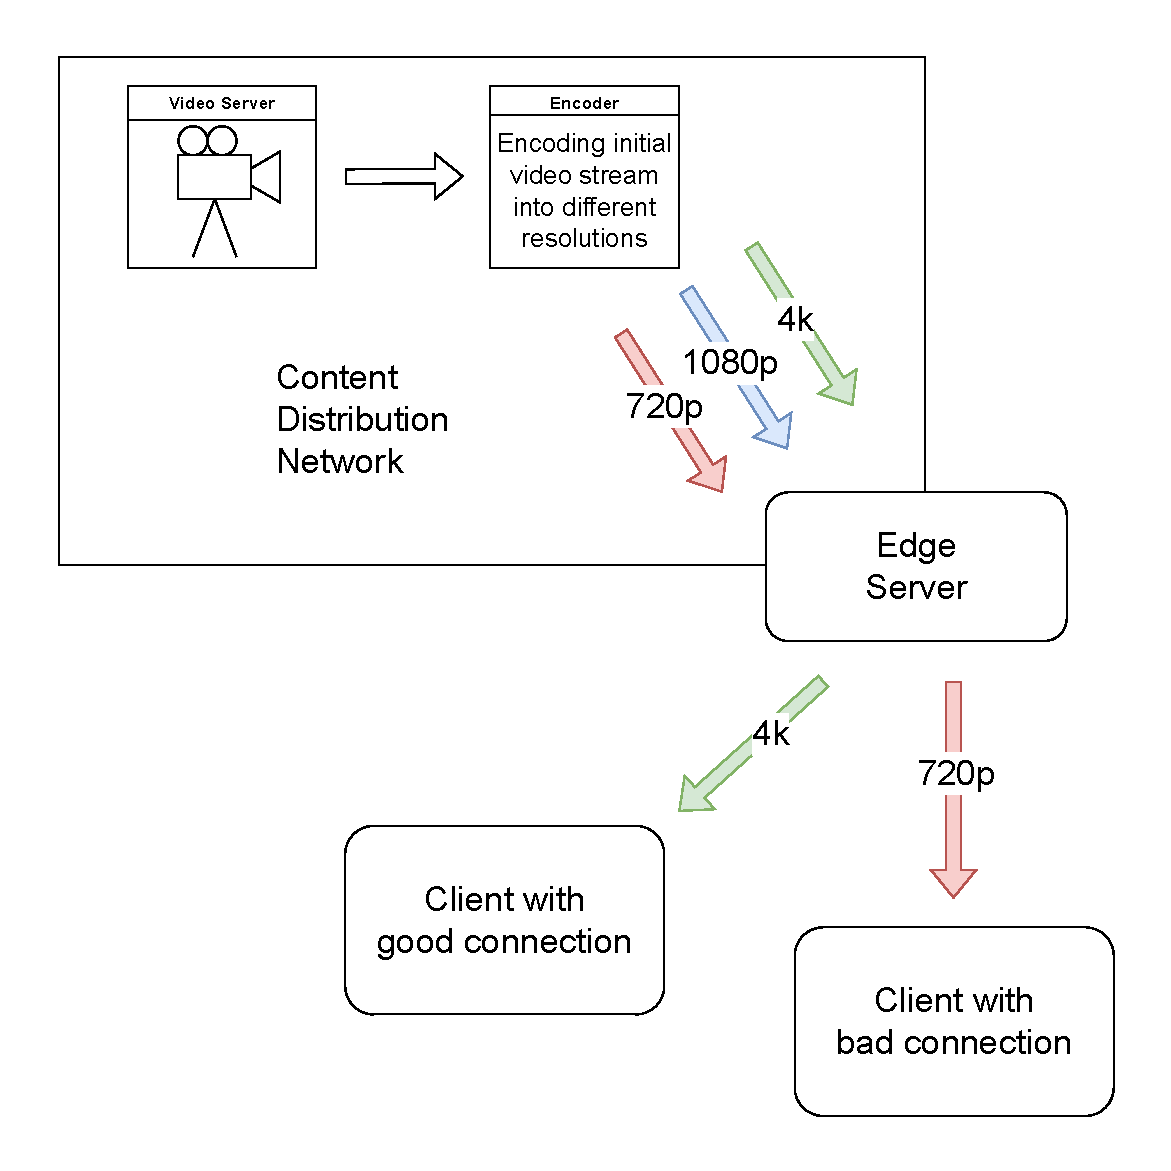
\includegraphics[width=\textwidth]{figures/02_background/adaptive-bitrate-streaming.drawio.pdf}
    \caption[Adaptive streaming schematic]{Behind the scenes multiple streams with different
    resolutions exists to allow adapting to a users bitrate.}\label{fig:adaptive-bitrate-streaming}
\end{figure}
% The way the example implementation of fast-realys in this thesis is set up,
% is that the video server will encode into each packet its priority.
% For example I-frames have a high priority while P-frames have a lower
% priority.
% The relay then can decide not to forward certain packets to a client if
% the client is experiencing congestion.
\vspace{1cm}

\subsection{Mechanisms and Ideas}
ABS implements the simple idea of chaning the amount of data sent to a client 
based on the clients connection quality.
This means a client with a good connection gets a higher quality stream than 
one with a bad connection.
For this the internal setup needs to be able to provide multiple streams with
different resolutions and bitrates.
An example setup can be seen in~\autoref{fig:adaptive-bitrate-streaming} where
an encoder creates streams with different resolutions and edge server, that 
manages the connections to the clients, can switch between those streams based 
the connection state of a specific client.
Youtube and Netflix are examples where, although more complex, similar setups
are used to provide a better user experience.
The premise of such a setup is that in case of a bad connection it is still 
preferable to be able to watch a stream contiuously, even if that means
cutting down on quality.

\subsection{Implications on Streaming Setup}
ABS forces a few changes to the way servers and relays are set up.
First, as figure~\autoref{fig:adaptive-bitrate-streaming} shows, there needs to 
be an ``encoding'' component that turns the single, high quality stream that is 
received from the streaming source into multiple streams with different resolutions.
Besides that the relay needs to keep track of the clients connection quality, e.g.~using 
measurements like RTT, packet loss, etc., and decide which stream to forward to the client.
Since the connection quality can change dynamically the relay also needs to continuously
monitor each connection and potentially change the used stream.
Besides encoding and monitoring aspects the system also has increased storage requirements
since stream data will essentially be duplicated.
